In this section we will further illustrate our framework by considering a different spacetime metric approximating an astrophysical binary black hole system referred to as the Superimposed Kerr-Schild solution, or SKS solution. The idea behind its construction is rather simple: One simply adds two Kerr solutions in Kerr-Schild coordinates and subtracts from this a Minkowski metric. After that, the black hole terms are further boosted and transformed in order to add motion to the individual black holes.

This prescription, of course, does not produce an exact solution of Einstein's field equations, nevertheless it can still be a valuable model for describing astrophysical binaries under certain conditions. The construction and motivation for using this approximation is extensively discussed in Refs.~\cite{Armengol:2021shd, PhysRevD.104.044041}, where it was  used in numerical simulations of accretion disks around BH binaries. Ref~\cite{Armengol:2021shd}, in particular, discusses the success of using superimposed solutions for computing initial data for numerical simulations of black hole mergers and shows that the expansion of the superimposed metric agrees with the lowest Post-Newtonian expansion of the metric of spinning binaries.

Furthermore, Ref.~\cite{PhysRevD.104.044041} compares the superimposed metric with other approximate solutions to binary black holes constructed with a much more mathematically involved technique called ``asymptotic matching'', that combines Post-Newtonian and other types of solutions in different regions of the spacetime and matches them together into a single solution. It shows that the violations of the Einstein field equations for the models constructed by matching and superposition are very similar in their order of magnitude and profile, with the matching solutions being more well-behaved and smooth at larger distances from the binary black holes. This leads them to conclude that given the mathematical simplicity of constructing a superimposed solution, they are more advantageous to matching solutions from a computational perspective.

Our ultimate aim is to demonstrate the applicability of the framework presented in this section to a wider range of spacetime metrics than the initial mathematical tool set utilized in the PP for static spacetimes. Our primary objective is not to provide quantitatively precise arguments about the behavior of the PP in astrophysical binaries. We only required a model in which two Kerr black holes follow a specific trajectory, breaking the time translation symmetry of the spacetime metric, and the SKS metric offers this model with greater ease than the PN matching counterparts.

Our construction of the SKS metric follows closely Refs.~\cite{Armengol:2021shd, PhysRevD.104.044041}, but we shall summarize the procedure here for the sake of clarity. We start by considering two Kerr metrics in Kerr-Schild coordinates $(T^{(i)}, X^{(i)}, Y^{(i)}, Z^{(i)})$ that describe each black hole, labeled by the index $(i) = 1,2$ and characterized by their masses $M^{(i)}$ and spin parameter $a^{(i)}$ in their rest frame. Let us now suppose there exists a global coordinate frame labeled by coordinates $(t,x,y,z)$ where the constituent black holes follow trajectories $s^{(i) \mu}(t, x, y, z)$. Following Ref.~\cite{Armengol:2021shd}, we will consider that the black holes follow a Keplerian orbit, given by
%
\begin{equation}
  s^{(i) \mu} = \left( (-1)^{i + 1}\frac{b}{2}\cos\Omega t,\, (-1)^{i + 1}\frac{b}{2}\sin\Omega t,\, 0 \right),
  \label{eq:arbitrary_penrose_sks_keplerian_trajectories}
\end{equation}
%
where
%
\begin{equation}
  \Omega = \sqrt{\frac{M^{(1)} + M^{(2)}}{b^3}}
  \label{eq:arbitrary_penrose_sks_angular_velocity}
\end{equation}
%
is the orbital angular velocity of the system and $b$ is the coordinate distance (in global coordinates) between the two black hole origins. From Eq.~\eqref{eq:arbitrary_penrose_sks_keplerian_trajectories}, we can compute the black hole velocity vector $v^{(i)} \mu = \ud s^{(i) \mu} / \ud t$ and obtain
%
\begin{equation}
  v^{(i) \mu} = \left( (-1)^i \frac{b\Omega}{2} \sin \Omega t,\, (-1)^{i+1} \frac{b\Omega}{2} \cos\Omega t,\, 0 \right),
  \label{eq:arbitrary_penrose_sks_keplerian_velocities}
\end{equation}
%
which can be normalized to yield
%
\begin{equation}
  n^{(i) \mu} = \left( (-1)^i \sin\Omega t,\, (-1)^{i+1}\cos\Omega t,\, 0 \right)
  \label{eq:arbitrary_penrose_sks_keplerian_velocities_norms}
\end{equation}
%
with norm
%
\begin{equation}
  v^2 \equiv \sum_{\mu = 0}^{2} v^{(i) \mu} = \frac{b^2 \Omega^2}{4}.
  \label{eq:arbitrary_penrose_sks_keplerian_velocities_norm}
\end{equation}
%
With these quantities, we can see that the Lorentz factor, $\gamma$, is given by
%
\begin{equation}
  \gamma \equiv \frac{1}{\sqrt{1 - v^2}} = \frac{2}{\sqrt{4 - b^2\Omega^2}}.
  \label{eq:arbitrary_penrose_sks_keplerian_orbit_lorentz_factor}
\end{equation}
%
It is then trivial to compute the generalized Lorentz boost of the trajectories
%
\begin{equation}
  \tens{\Lambda}{(i) \mu}{\nu} =
  \begin{pmatrix}
    \gamma            & -\gamma v^{(i) 0}              & -\gamma v^{(i) 1}              & 0 \\
    -\gamma v^{(i) 0} & 1+(\gamma-1) n^{(i)0} n^{(i)0} & (\gamma-1) n^{(i)0} n^{(i)1}   & 0 \\
    -\gamma v^{(i) 1} & (\gamma-1)n^{(i)1} n^{(i)0}    & 1+(\gamma-1) n^{(i)1} n^{(i)1} & 0 \\
    0                 & 0                              & 0                              & 1
  \end{pmatrix}
  \label{eq:arbitrary_penrose_sks_lorentz_boost}
\end{equation}
%
by virtue of Eqs.~\eqref{eq:arbitrary_penrose_sks_keplerian_velocities}-\eqref{eq:arbitrary_penrose_sks_keplerian_orbit_lorentz_factor}. The next step of the construction, is therefore, to boost each individual Kerr metric using Eq.~\eqref{eq:arbitrary_penrose_sks_lorentz_boost}. We remind the reader that the Kerr-Schild form of the metric is maintained after a Lorentz boost. Finally, we must transform each local coordinate of each individual black hole to global coordinates. This is done via a non-linear coordinate transformation (or a ``circular boost'', as Ref.~\cite{Armengol:2021shd} puts it) that reads
%
\begin{align}
  t & = \gamma \left( T - v^{(i) 0} X - v^{(i) 1} Y \right) \label{eq:arbitrary_penrose_sks_nonlinear_transformation_1}                                                                                          \\
  x & = s^{(i) 0} + X \left[ 1 + \left( \gamma - 1 \right) n^{(i) 0} n^{(i) 0}\right] + Y \left[\left( \gamma - 1 \right) n^{(i) 0} n^{(i) 1}\right] \label{eq:arbitrary_penrose_sks_nonlinear_transformation_2} \\
  y & = s^{(i) 1} + X \left[\left( \gamma - 1 \right) n^{(i) 0} n^{(i) 1}\right] + Y \left[1 + \left( \gamma - 1 \right) n^{(i) 1} n^{(i) 1}\right]  \label{eq:arbitrary_penrose_sks_nonlinear_transformation_3} \\
  z & = Z \label{eq:arbitrary_penrose_sks_nonlinear_transformation_4}
\end{align}

To summarize, the algorithm one must employ in order to construct the SKS metric in global coordinates $(t,x,y,z)$ with black holes that are following the Keplerian trajectories given by Eq.~\eqref{eq:arbitrary_penrose_sks_keplerian_trajectories} and possess mass and spin parameters $M^{(1,2)}$ and $a^{(1,2)}$, respectively, and coordinate separation $b$ is as follows:
%
\begin{enumerate}
  \item Compute the value of $\Omega$ from the metric parameters (masses and separation) via Eq.~\eqref{eq:arbitrary_penrose_sks_angular_velocity}.
  \item Compute $\gamma$ via Eq.~\eqref{eq:arbitrary_penrose_sks_keplerian_orbit_lorentz_factor}.
  \item Compute each component of the trajectory velocity vector $v^{(i) \mu}$ and normal vector $n^{(i) \mu}$ via Eqs.~\eqref{eq:arbitrary_penrose_sks_keplerian_velocities} and \eqref{eq:arbitrary_penrose_sks_keplerian_velocities_norms}, respectively.
  \item Construct the Lorentz boost matrix via Eq.~\eqref{eq:arbitrary_penrose_sks_lorentz_boost}.
  \item Boost the ``black hole part'' of the Kerr-Schild metric, that is, replace  $\mathcal{M}_{\mu\nu} = H l_\mu l_\nu$ by $\overline{\mathcal{M}}^{(i)}_{\mu\nu} = H^{(i)} \tens{\Lambda}{(i) \alpha}{\mu} \tens{\Lambda}{(i) \beta}{\nu} l^{(i)}_\alpha l^{(i)}_\beta$ for each black hole.
  \item Find the coordinate values $(T^{(i)}, X^{(i)}, Y^{(i)}, Z^{(i)})$ for each black hole by inverting the system formed by Eqs.~\eqref{eq:arbitrary_penrose_sks_nonlinear_transformation_1}-\eqref{eq:arbitrary_penrose_sks_nonlinear_transformation_4}.
  \item Substitute $(T^{(i)}, X^{(i)}, Y^{(i)}, Z^{(i)})$ into $\overline{\mathcal{M}}^{(i)}_{\mu\nu}$, producing $\overline{\mathcal{H}}^{(i)}_{\mu\nu}(t,x,y,z)$.
  \item The final metric components are given by $\mtrtens{\mu}{\nu}(t,x,y,z) = \eta_{\mu\nu} + \overline{\mathcal{H}}^{(1)}_{\mu\nu} + \overline{\mathcal{H}}^{(2)}_{\mu\nu}$.
\end{enumerate}

We have implemented the SKS solution as a plugin in \texttt{GRLensing} and validated the implementation by comparing plots of the metric components against the results of Ref.~\cite{PhysRevD.104.044041}. We have also constructed the metric analytically using a \texttt{Mathematica} notebook that was also used in order to independently check the components as implemented in the \texttt{C++} code and cross-check those results against Ref.~\cite{PhysRevD.104.044041}. Furthermore, we have also used this notebook to identify the region where the $\mtrtens{t}{t}$ component changes its sign. This region can be understood as the ``ergosphere'' viewed by an observer living in the global reference frame labeled by $(t,x,y,z)$. Note however, that strictly speaking the use of the word ``ergosphere'' in this context is an abuse, since it refers to a region that is globally defined via the existence of the time-like killing vector field. Nevertheless, we can observe this region as the spacetime metric parameters change, similarly to our work in Sections \ref{ch:penrose_binaries:sec:mp_penrose} and \ref{ch:penrose_binaries:sec:cmmr_penrose}. The general features of the local ergosphere in the SKS metric resemble that of the CMMR metric, presented in Sec.~\ref{ch:penrose_binaries:sec:cmmr_penrose}, with the remarkable difference that the Lorentz boosts required for the construction of the SKS spacetime make the ergospheres ``flattened'' the direction of the motion of the holes. This is a well-known effect that can be observed even in the Schwarzschild spacetime, as demonstrated in Ref.~\cite{PhysRevD.91.084044}. Fig.~\ref{fig:sks_ergo_plot} illustrates relevant regions in the SKS spacetime with black holes masses $M^{(1)} = M^{(2)} = 1/2$, spin parameters $a^{(1)} = a^{(2)} = 1/4$ and separation parameter $b = 3$. The boundary of the local ergosphere is marked in red, the approximate location of the event horizons in gray, the singular region in black and the black hole centers are indicated by black crosshairs. As was previously mentioned, the boundary of the ergosphere is marked as the surface where the $\mtrtens{t}{t}$ component changes its sign. The event horizons and singular regions are given by~\cite{Armengol:2021shd}
%
\begin{equation}
  r^{(1,2)} = 2 M^{(1,2)} \left( M^{(1,2)} + \sqrt{M^{(1,2)} - \left(a^{(1,2)}\right)^2} \right)
  \label{eq:arbitrary_penrose_sks_keplerian_approx_horizons}
\end{equation}
%
and
%
\begin{equation}
  r^{(1,2)} = \left| a^{(1,2)} \right|,
  \label{eq:arbitrary_penrose_sks_keplerian_approx_singularities}
\end{equation}
%
respectively, where $r^{(1,2)}$ is the coordinate distance measured from one of the black hole centers. The figure shows that the ergosphere gets ``dragged along'' the direction of motion of the black holes.

\begin{figure}[!ht]
  \centering
  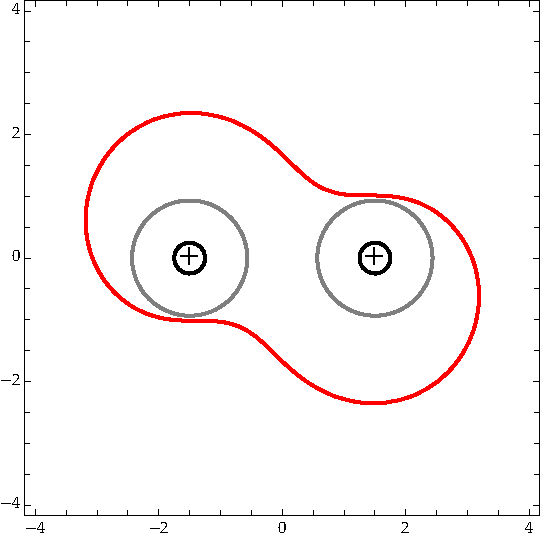
\includegraphics[width=\linewidth]{img/penrose_binaries/sks_regions.pdf}
  \caption{Regions of interest in the SKS metric. The red region marks the boundary of the local ergosphere while the gray and black regions mark, respectively, the event horizons and singularities. The black crosshairs mark the centers of the black holes. The spacetimes parameters were chosen to be $M^{(1)} = M^{(2)} = 1/2$, $a^{(1)} = a^{(2)} = 1/4$ and $b = 3$}
  \label{fig:sks_ergo_plot}
\end{figure}

\subsubsection{Example 1}
\label{ch:sks_example_1}

For our first example, we have chosen the system parameters as $M^{(1)} = M^{(2)} = 1/2$, $a^{(1)} = a^{(2)} = 0.49$ and $b = 10$. The break-up point was chosen at coordinates $X^i = (6.3, 0, 0)$ and the background sphere radius was chosen to be $1.0 \times 10^6$. Following the same template of Table~\ref{tab:arbitrary_penrose_kerr_example_energy_mass}, Table~\ref{tab:arbitrary_penrose_sks_example_energy_mass} summarizes the initial energy and mass of the participating particles. Once again, the first, second and third rows contain data relative to the entry, Penrose and exit orbits, respectively. The parameters for the entry and Penrose orbits are chosen explicitly via configuration file fed to the code, while the parameters of the exit orbit are computed via the conservation of 4-momentum at the break-point. The masses are explicitly chosen in order to satisfy Eq.~\eqref{eq:mass_constraint} and to provide a way of computing initial velocities via Eqs.~\eqref{eq:arbitrary_penrose_ellipse_parametric_1}-\eqref{eq:arbitrary_penrose_ellipse_parametric_2}
%
\begin{table}[]
  \centering
  \begin{tabular}{cc}
    \hline\hline
    $E(0)$                              & $m$                                 \\
    $1.0$                               & $1.0 \times 10^{-1}$                \\
    $8.0 \times 10^{-3}$                & $1.0 \times 10^{-4}$                \\
    $9.9199999999999999 \times 10^{-1}$ & $9.5800493929022838 \times 10^{-3}$ \\ \hline\hline
  \end{tabular}
  \caption{Initial energy and masses for the particles participating in the PP example. The first two rows are given explicitly via configuration value and represent the ingoing and Penrose trajectories, respectively. The third row represents the exit trajectory and is computes via conservation of 4-momentum.}
  \label{tab:arbitrary_penrose_sks_example_energy_mass}
\end{table}

Once more, following Table~\ref{tab:arbitrary_penrose_kerr_example_velocities}, Table~\ref{tab:arbitrary_penrose_sks_example_velocities} summarizes the initial velocities of the participating particles. Here, the values of the first two rows (representing the ingoing and Penrose trajectories, respectively), were computed via the parametrization described in the previous section together with data from Tab.~\ref{tab:arbitrary_penrose_kerr_example_energy_mass} while data on the third row, representing the outgoing particle, was computed via conservation of 4-momentum. The third column in this table shows the value of the ellipse parameter chosen for each orbit (except the exit orbit).
%
\begin{table}[]
  \centering
  \begin{tabular}{ccc}
    \hline\hline
    $V^x(0)$              & $V^y(0)$              & $\Theta$       \\
    $0.6769503786998466$  & $0.6740022058848380$  & $-25/200 \pi$  \\
    $0.5948571400034293$  & $-0.3343724878526367$ & $-100/200 \pi$ \\
    $0.66011565390809868$ & $0.68380243736284951$ & ---            \\ \hline\hline
  \end{tabular}
  \caption{Initial velocities for the particles participating in the PP example. The first two rows are computed using the ellipse parametrization described in the previous section with data provided in Tab.~\ref{tab:arbitrary_penrose_sks_example_energy_mass} together with the parameter provided in the third column and represent the ingoing and Penrose trajectories, respectively. The third row represents the exit trajectory and is computes via conservation of 4-momentum.}
  \label{tab:arbitrary_penrose_sks_example_velocities}
\end{table}

As Table~\ref{tab:arbitrary_penrose_kerr_example_results}, Table~\ref{tab:arbitrary_penrose_sks_example_results} summarizes the two energy measures (local and global on the first and second column, respectively) at the time when they hit the background sphere. The first row contains data relative to the ingoing orbit while the second contains data relative to the outgoing orbit. Note that $t_f$ does not necessarily coincide for the two orbits, since they might take arbitrarily long paths before escaping to infinity. The third column shows the absolute difference between global and local energies at the background sphere.
%
\begin{table}[]
  \centering
  \resizebox{\textwidth}{!}{
    \begin{tabular}{ccc}
      \hline\hline
      $E(t_f)$                            & $\varepsilon(t_f)$                  & $|E(t_f) - \varepsilon(t_f)|$       \\
      $2.4452985315377770 \times 10^{-1}$ & $2.4453006741751246 \times 10^{-1}$ & $2.1426373481014949 \times 10^{-7}$ \\
      $3.4638508542318119 \times 10^{-1}$ & $3.4638400572434974 \times 10^{-1}$ & $1.0796988314520917 \times 10^{-6}$ \\ \hline\hline
    \end{tabular}
  }
  \caption{Energy measures at the time of collision with the background sphere. The first and second row represent the ingoing and the outgoing orbits, respectively. The third column shows the absolute difference between energy measures at the background sphere radius. Note that $t_f$ is not necessarily the same for both trajectories.}
  \label{tab:arbitrary_penrose_sks_example_results}
\end{table}

Finally, following Table~\ref{tab:arbitrary_penrose_kerr_example_efficiency}, Table~\ref{tab:arbitrary_penrose_sks_example_efficiency} summarizes the amount of energy extracted from the process in different forms. The first and second rows compute the difference between the energy of the outgoing and ingoing particles using different energy measures (local and global respectively). Since this difference is positive, we can conclude that energy was indeed extracted from the black hole. The last two rows compute the efficiency of the process for the two available energy measures, given by Eq~\eqref{eq:arbitrary_penrose_kerr_example_efficiency_formula}.
\begin{table}[]
  \centering
  \begin{tabular}{cc}
    \hline\hline
    $E_\text{out}(t_f)-E_\text{in}(t_f)$                     & $0.10185523226940352$ \\
    $\varepsilon_\text{out}(t_f)-\varepsilon_\text{in}(t_f)$ & $0.10185393830683726$ \\
    $\eta_E$                                                 & $0.41653495863897544$ \\
    $\eta_\varepsilon$                                       & $0.41652966700464295$ \\ \hline\hline
  \end{tabular}
  \caption{Energy difference and extraction efficiency of the process given different energy measures.}
  \label{tab:arbitrary_penrose_sks_example_efficiency}
\end{table}

\subsubsection{Example 2}
\label{ch:sks_example_2}

In this example, we repeat the run detailed in Sec.~\ref{ch:sks_example_1} while changing the distance parameter from $b=10.0$ to $b = 7.21$. We have also changed the break-up point coordinates in each run so that it remains at $1.3$ coordinate distance units to the right of the right-most black hole. The results of this variation are summarized in Table~\ref{tab:arbitrary_penrose_sks_example_results_d_variation} where it is possible to see that the efficiency decreases as the black wholes get more distant from each other.

\begin{table}[]
  \centering
  \begin{tabular}{ccc}
    \hline\hline
    $d$  & $\eta_E$             & $\eta_\varepsilon$   \\
    10.0 & $0.4165349586389754$ & $0.4165293020302941$ \\
    9.69 & $0.4099912589653710$ & $0.4099855399919209$ \\
    9.38 & $0.4042822480170929$ & $0.4042767439403118$ \\
    9.07 & $0.3994849072973370$ & $0.3994792027270561$ \\
    8.76 & $0.3954568832639254$ & $0.3954513766173146$ \\
    8.45 & $0.3915618006432178$ & $0.3915564144708418$ \\
    8.14 & $0.3857189791093659$ & $0.3857135001267253$ \\
    7.83 & $0.3709406424619314$ & $0.3709350873643125$ \\
    7.52 & $0.3205512719659607$ & $0.3205458837844264$ \\
    7.21 & $0.1207168410527975$ & $0.1207122709189437$ \\ \hline\hline
  \end{tabular}
  \caption{Energy extraction efficiency for the configuration detailed in Sec~\ref{ch:sks_example_1} while varying the distance parameter $b$ and keeping the break-up point at $1.3$ coordinate distance unites to the right of the rightmost black hole.}
  \label{tab:arbitrary_penrose_sks_example_results_d_variation}
\end{table}

\subsubsection{Example 3}
\label{ch:sks_example_3}

In this example we vary the mass of the left-most black hole $M^{(2)}$ from $0.5$ to $0.275$ while also changing the spin parameter according to $a^{(2)} = 0.98 M^{(2)}$. We keep fixed the mass $M^{(1)} = 0.5$, the spin parameter $a^{(1)} = 0.49$, the distance parameter $b=20.0$ and the break-up point $(11.0, 0.0, 0.0)$. This configuration is analogue to that of the single Kerr black hole example of Sec.~\ref{ch:kerr_example}. The results are summarized in Table~\ref{tab:arbitrary_penrose_sks_example_results_M2_variation}, where it is possible to see that as the mass of the companion black hole decreases, the extraction efficiency decreases.

\begin{table}[]
  \centering
  \begin{tabular}{ccc}
    \hline\hline
    $M2$  & $\eta_E$             & $\eta_\varepsilon$   \\
    0.500 & $0.1057279994029897$ & $0.1057236710602922$ \\
    0.475 & $0.0870377969920106$ & $0.0870336429442202$ \\
    0.450 & $0.0712047949044382$ & $0.0712008663973118$ \\
    0.425 & $0.0578255784926676$ & $0.0578218053066227$ \\
    0.400 & $0.0465203386664686$ & $0.0465166569217887$ \\
    0.375 & $0.0369572283763885$ & $0.0369537431441037$ \\
    0.350 & $0.0288551456052595$ & $0.0288518045002344$ \\
    0.325 & $0.0219792546154663$ & $0.0219759777138235$ \\
    0.300 & $0.0161341223097530$ & $0.0161310745614111$ \\
    0.275 & $0.0111575173287062$ & $0.0111545996429916$ \\ \hline\hline
  \end{tabular}
  \caption{Energy extraction efficiency for fixed mass $M^{(1)} = 0.5$, spin parameter $a^{(1)} = 0.49$, distance parameter $b=20.0$ and break-up point $(11.0, 0.0, 0.0)$ and varying Mass $M^{(2)}$ and spin parameter $a^{(2)} = 0.98 M^{(2)}$.}
  \label{tab:arbitrary_penrose_sks_example_results_M2_variation}
\end{table}